\section{KITTI}

Using ShapeNet \cite{ChangFunkhouserGuibasSavarese:2015} we are able to learn
a shape prior enabling us to perform shape completion on KITTI
\cite{GeigerLenzUrtasun:2012,GeigerLenzStillerUrtasun:2013}.
On KITTI, however, we do not have access to ground truth shapes.
We found that manual annotation (\eg following \cite{MenzeGeiger:2015}) 
would go far beyond the time frame of this thesis. Still,
we intend to provide insightful experiments thereby, again, focusing on
\AML using both modalities, \ie occupancy and signed distance functions.
Our goal is to demonstrate that \AML is able to predict reasonable
shapes given the noisy observations from KITTI's Velodyne sensor.

Following the discussion in Section \ref{sec:data-kitti}, we filtered
the provided ground truth 3D bounding boxes using $n_{1,\min} = 150$,
$n_{0,\min} = 1500$ and $t_{\max} = 30$. This means, that we require at least
$150$ voxels to be observed as occupied and $1500$ observed voxels
to correspond to free space. Additionally, we only consider bounding boxes
within $30m$ of the sensor. Overall, we obtained $1928$ distinct car observations
which we split into a training set with $1714$ and a validation with
$214$ samples.
On average, $\sim 0.634\%$ of voxels are observed points; $\sim 5.98\%$
of voxels are free space. In this regard, the dataset might be slightly
easier than the \hard ShapeNet dataset, where only $0.304\%$ of voxels are
observed as being occupied. In spite of these strict requirements regarding
the number of observed voxels, we find the extracted dataset to be particularly
challenging due to the corresponding noise patterns. We show additional examples
of the dataset in Appendix \ref{ch:appendix-data}.
% TODO examples!

\subsection{Amortized Maximum Likelihood}

\begin{figure}
  \centering
  \begin{tikzpicture}
    \node at (0, 0){
      \includegraphics[width=6cm]{experiments/kitti/vae_occ_aml/15_long/results_1}
    };
    \node at (0, -2.5){
      \includegraphics[width=6cm]{experiments/kitti/vae_occ_aml/15_long_statistics/results_1}
    };
    \node at (0, -5){
      \includegraphics[width=6cm]{experiments/kitti/vae_occ_aml/15_long_statistics_combined/results_1}
    };
   
    \node at (6.25, 0){
      \includegraphics[width=6cm]{experiments/kitti/vae_occ_aml/15_long/results_4}
    };
    \node at (6.25, -2.5){
      \includegraphics[width=6cm]{experiments/kitti/vae_occ_aml/15_long_statistics/results_4}
    };
    \node at (6.25, -5){
      \includegraphics[width=6cm]{experiments/kitti/vae_occ_aml/15_long_statistics_combined/results_4}
    };
    
    \draw[-,dashed] (-3.25, -1.25) -- (9.5,-1.25);
    \draw[-,dashed] (-3.25, -3.75) -- (9.5,-3.75);
    
    %\node at (10,0) {
    %  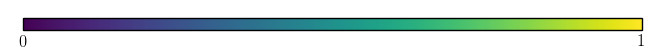
\includegraphics[height=2.5cm]{experiments/3d/vae_occ/easy_15/colorbar}
    %};
    
    \node at (3.25, 1.5) {reconstruction};
    \node[rotate=90] at (-3.5, 0) {\AML};
    \node[rotate=90] at (-3.75, -2.5) {\begin{tabular}{c}\AML\\+weights\end{tabular}};
    \node[rotate=90] at (-4, -5) {\begin{tabular}{c}\AML\\+weights\\+combined\end{tabular}};
  \end{tikzpicture}

  % TODO short caption
  \caption{Qualitative results for \AML on the extracted KITTI dataset. We demonstrate
  the influence of using the weights $\rho_i$ marked as +weights; here, the weights are
  pre-computed on ShapeNet as discussed for Equation \eqref{eq:experiments-3d-weights}.
  Additionally we show the influence of training the prior on both ShapeNet training sets,
  referred to as +combined. As always, we show horizontal slices for the observed points,
  the corresponding partial free space and the predictions.
  }
  \label{fig:experiments-kitti-aml-1}
\end{figure}

\begin{figure}
  \centering
  %\hspace*{-1.5cm}
  \begin{tikzpicture}
    \node at (0, 0) {
      \includegraphics[width=3.75cm,trim={3.5cm 2.5cm 3.5cm 2.5cm},clip]{experiments/kitti/vae_occ_aml/15_long_statistics_combined/0_input_45}
    };
    \node at (3.5, 0) {
      \includegraphics[width=3.75cm,trim={3.5cm 2.5cm 3.5cm 2.5cm},clip]{experiments/kitti/vae_occ_aml/15_long_statistics_combined/0_prediction_45}
    };
    \node at (7, 0) {
      \includegraphics[width=3.75cm,trim={3.5cm 2.5cm 3.5cm 2.5cm},clip]{experiments/kitti/baseline/moderate_15/0_prediction_45}
    };

    % \node at (7, 0) {
    %   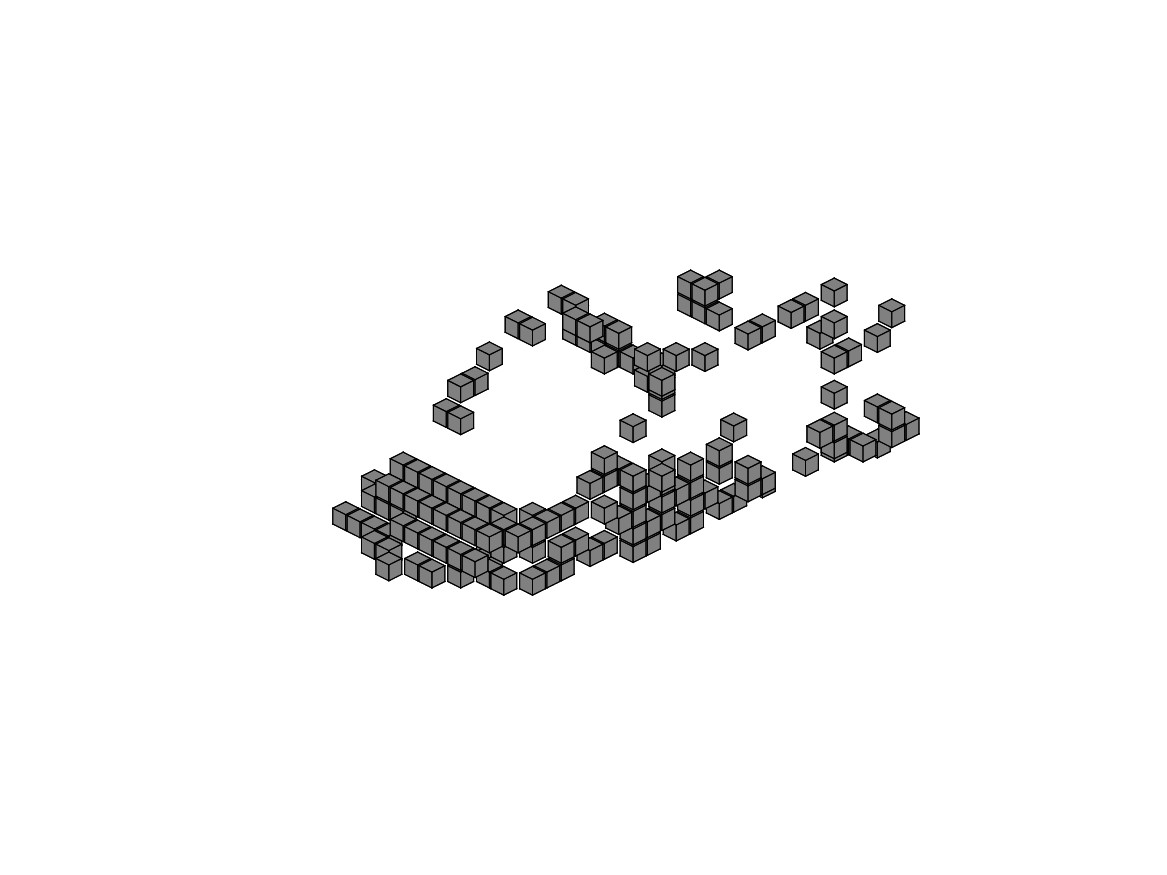
\includegraphics[width=3.75cm,trim={3.5cm 2.5cm 3.5cm 2.5cm},clip]{experiments/kitti/vae_occ_aml/15_long_statistics_combined/2_input_135}
    % };
    % \node at (10.5, 0) {
    %   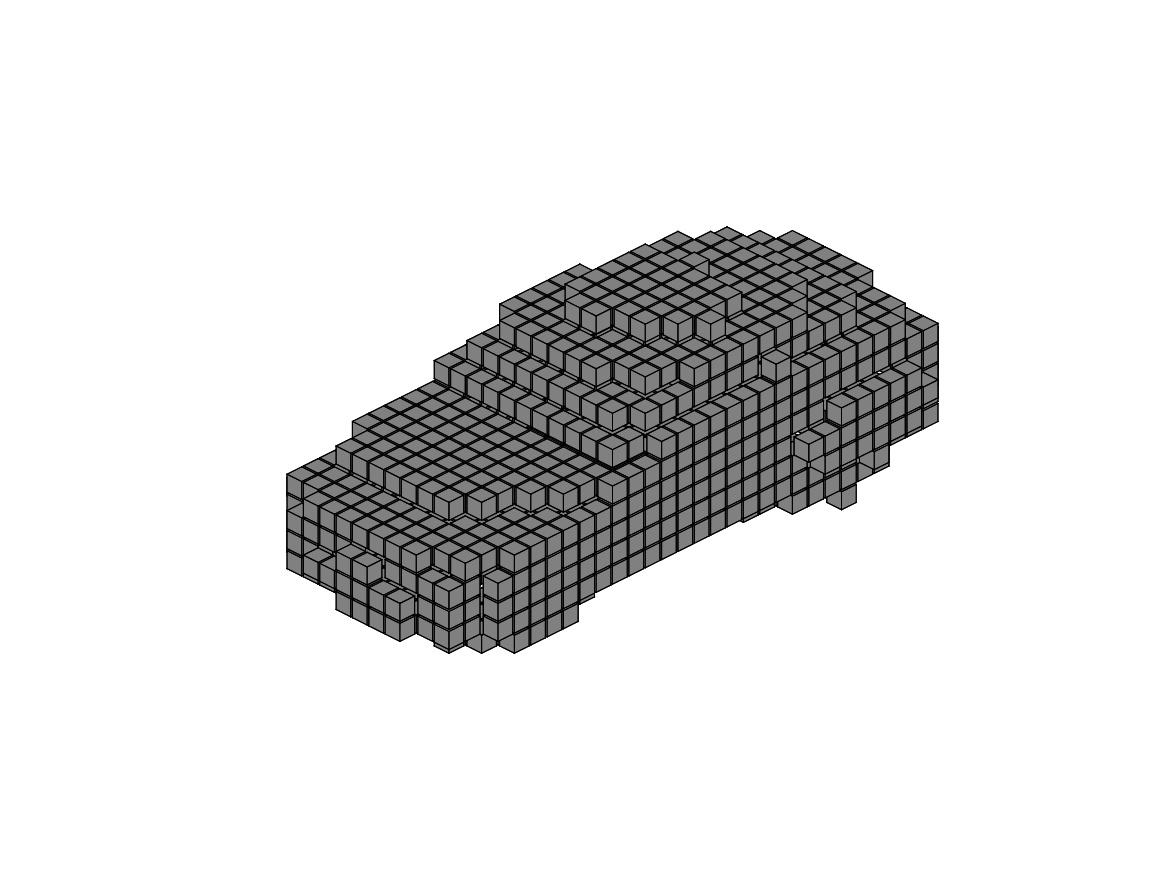
\includegraphics[width=3.75cm,trim={3.5cm 2.5cm 3.5cm 2.5cm},clip]{experiments/kitti/vae_occ_aml/15_long_statistics_combined/2_prediction_135}
    % };
    
    \node at (0, -3) {
      \includegraphics[width=3.75cm,trim={3.5cm 2.5cm 3.5cm 2.5cm},clip]{experiments/kitti/vae_occ_aml/15_long_statistics_combined/1_input_45}
    };
    \node at (3.5, -3) {
      \includegraphics[width=3.75cm,trim={3.5cm 2.5cm 3.5cm 2.5cm},clip]{experiments/kitti/vae_occ_aml/15_long_statistics_combined/1_prediction_45}
    };
    \node at (7, -3) {
      \includegraphics[width=3.75cm,trim={3.5cm 2.5cm 3.5cm 2.5cm},clip]{experiments/kitti/baseline/moderate_15/1_prediction_45}
    };

    % \node at (7, -3) {
    %   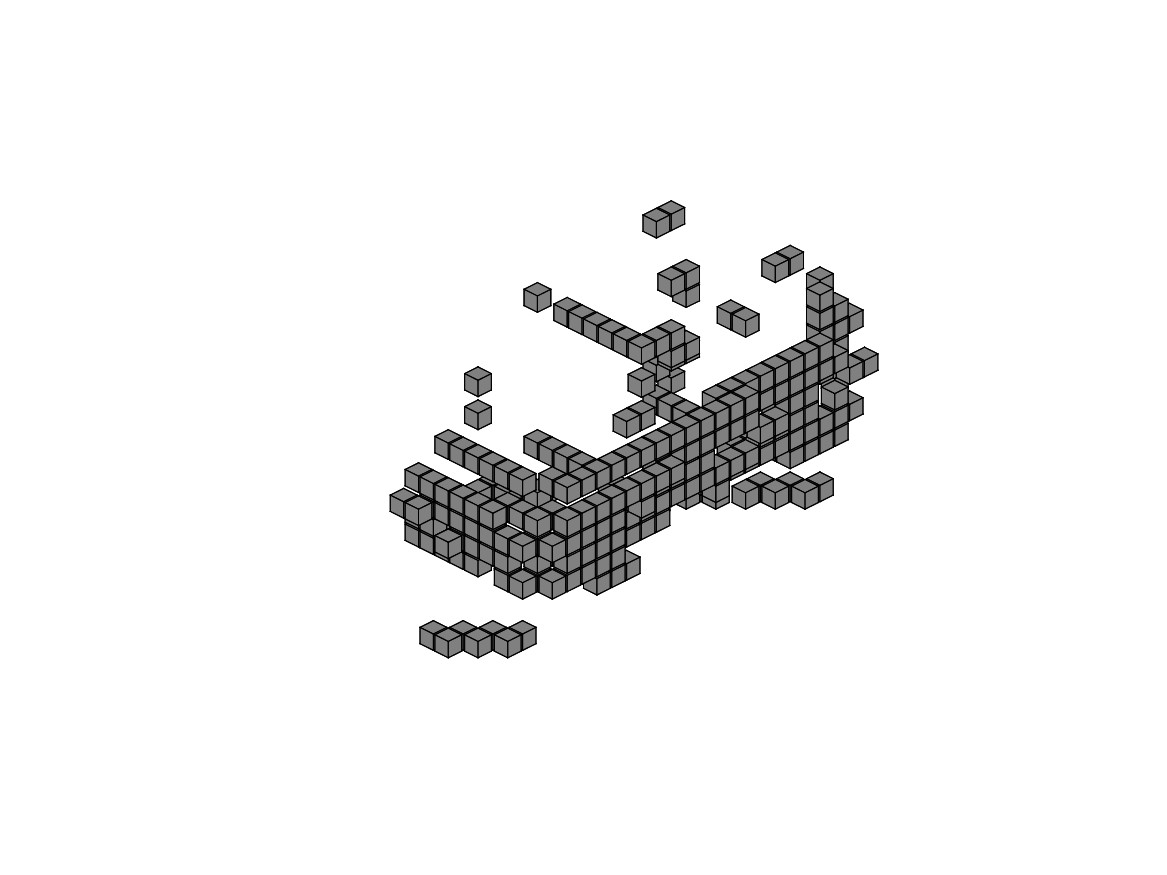
\includegraphics[width=3.75cm,trim={3.5cm 2.5cm 3.5cm 2.5cm},clip]{experiments/kitti/vae_occ_aml/15_long_statistics_combined/0_input_135}
    % };
    % \node at (10.5, -3) {
    %   \includegraphics[width=3.75cm,trim={3.5cm 2.5cm 3.5cm 2.5cm},clip]{experiments/kitti/vae_occ_aml/15_long_statistics_combined/0_prediction_135}
    % };
  
    \node at (0, -6) {
      \includegraphics[width=3.75cm,trim={3.5cm 2.5cm 3.5cm 2.5cm},clip]{experiments/kitti/vae_occ_aml/15_long_statistics_combined/2_input_45}
    };
    \node at (3.5, -6) {
      \includegraphics[width=3.75cm,trim={3.5cm 2.5cm 3.5cm 2.5cm},clip]{experiments/kitti/vae_occ_aml/15_long_statistics_combined/2_prediction_45}
    };
    \node at (7, -6) {
      \includegraphics[width=3.75cm,trim={3.5cm 2.5cm 3.5cm 2.5cm},clip]{experiments/kitti/baseline/moderate_15/2_prediction_45}
    };

    % \node at (7, -6) {
    %   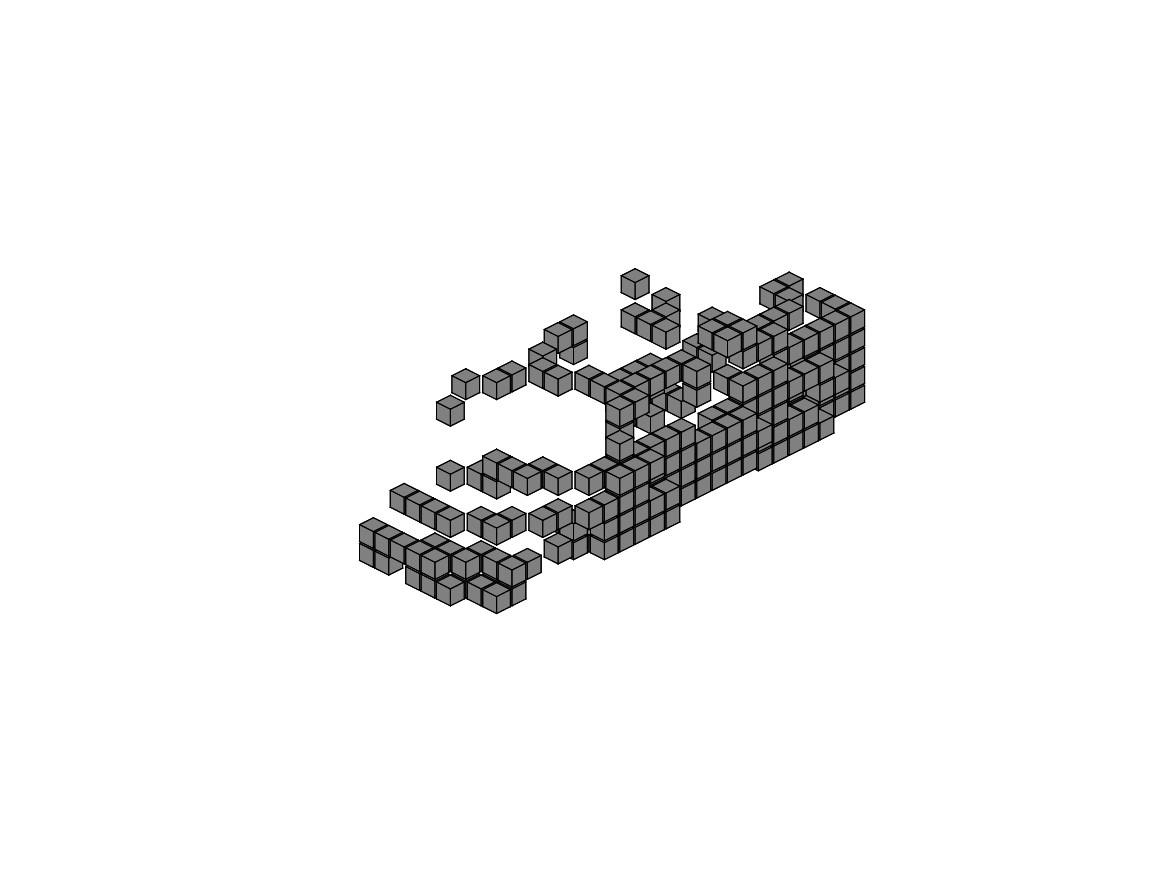
\includegraphics[width=3.75cm,trim={3.5cm 2.5cm 3.5cm 2.5cm},clip]{experiments/kitti/vae_occ_aml/15_long_statistics_combined/1_input_135}
    % };
    % \node at (10.5, -6) {
    %   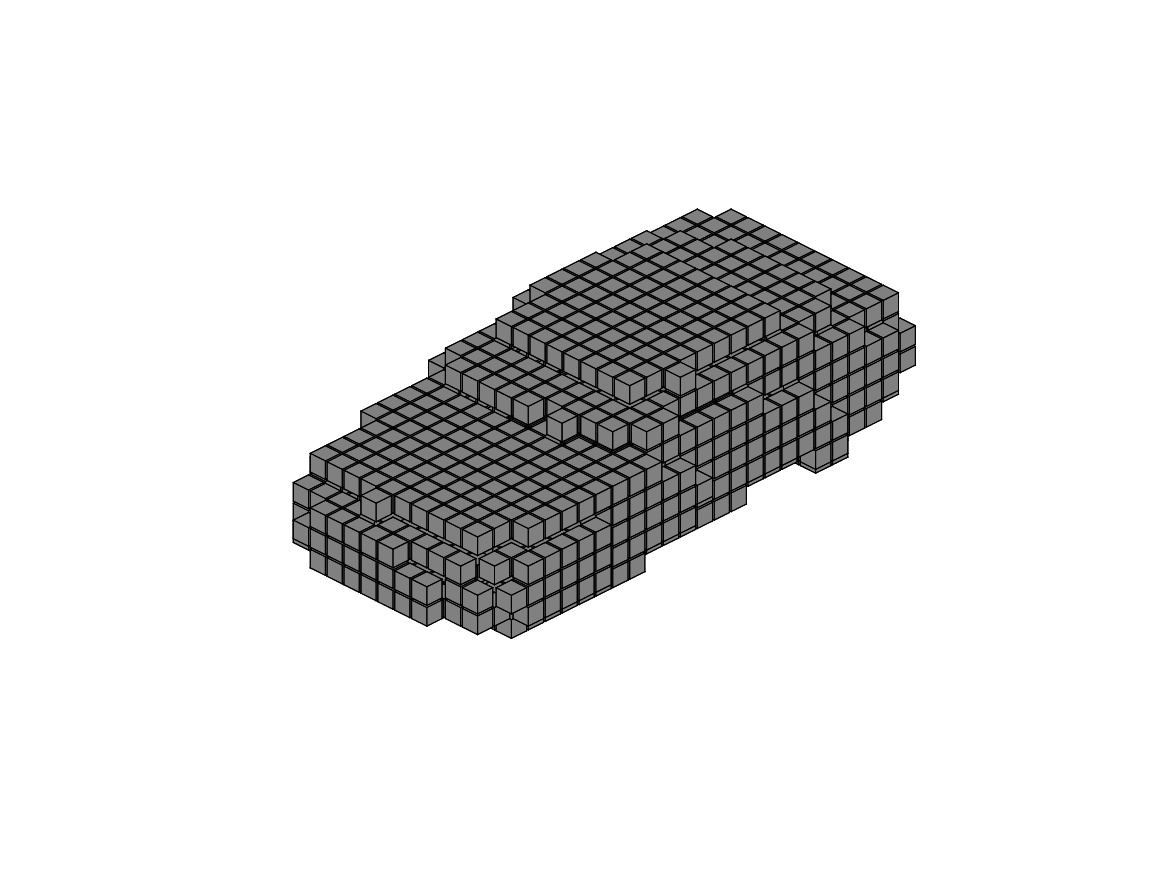
\includegraphics[width=3.75cm,trim={3.5cm 2.5cm 3.5cm 2.5cm},clip]{experiments/kitti/vae_occ_aml/15_long_statistics_combined/1_prediction_135}
    % };
    
    \node at (0, -9) {
      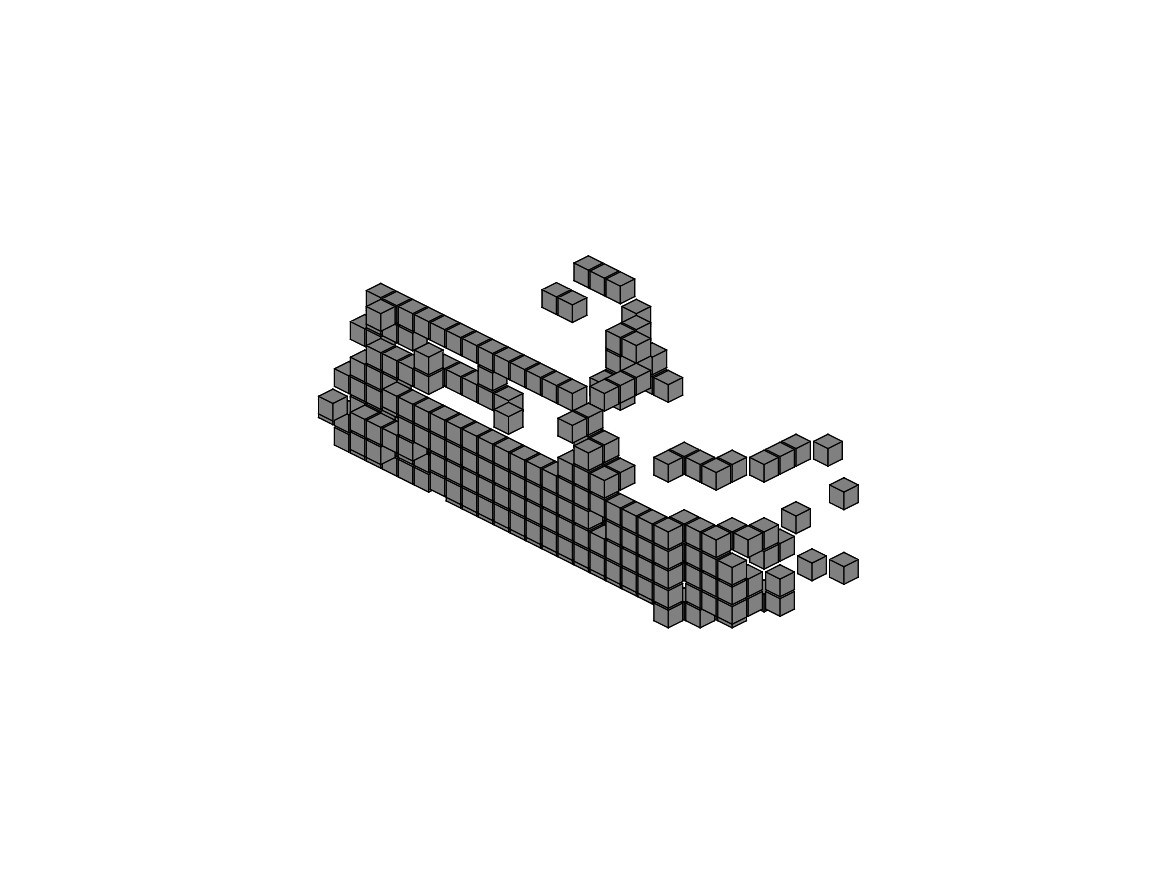
\includegraphics[width=3.75cm,trim={3.5cm 2.5cm 3.5cm 2.5cm},clip]{experiments/kitti/vae_occ_aml/15_long_statistics_combined/3_input_45}
    };
    \node at (3.5, -9) {
      \includegraphics[width=3.75cm,trim={3.5cm 2.5cm 3.5cm 2.5cm},clip]{experiments/kitti/vae_occ_aml/15_long_statistics_combined/3_prediction_45}
    };
    \node at (7, -9) {
      \includegraphics[width=3.75cm,trim={3.5cm 2.5cm 3.5cm 2.5cm},clip]{experiments/kitti/baseline/moderate_15/3_prediction_45}
    };

    % \node at (7, -9) {
    %   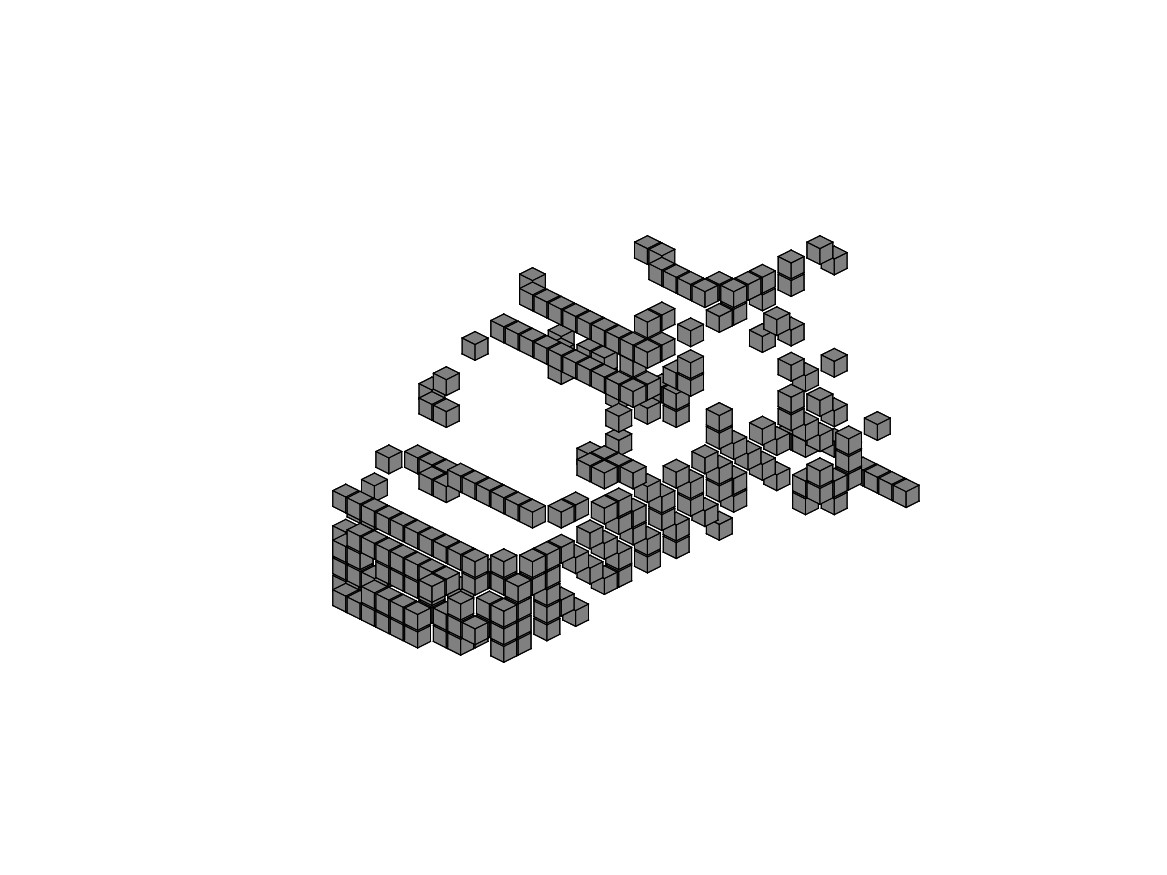
\includegraphics[width=3.75cm,trim={3.5cm 2.5cm 3.5cm 2.5cm},clip]{experiments/kitti/vae_occ_aml/15_long_statistics_combined/4_input_135}
    % };
    % \node at (10.5, -9) {
    %   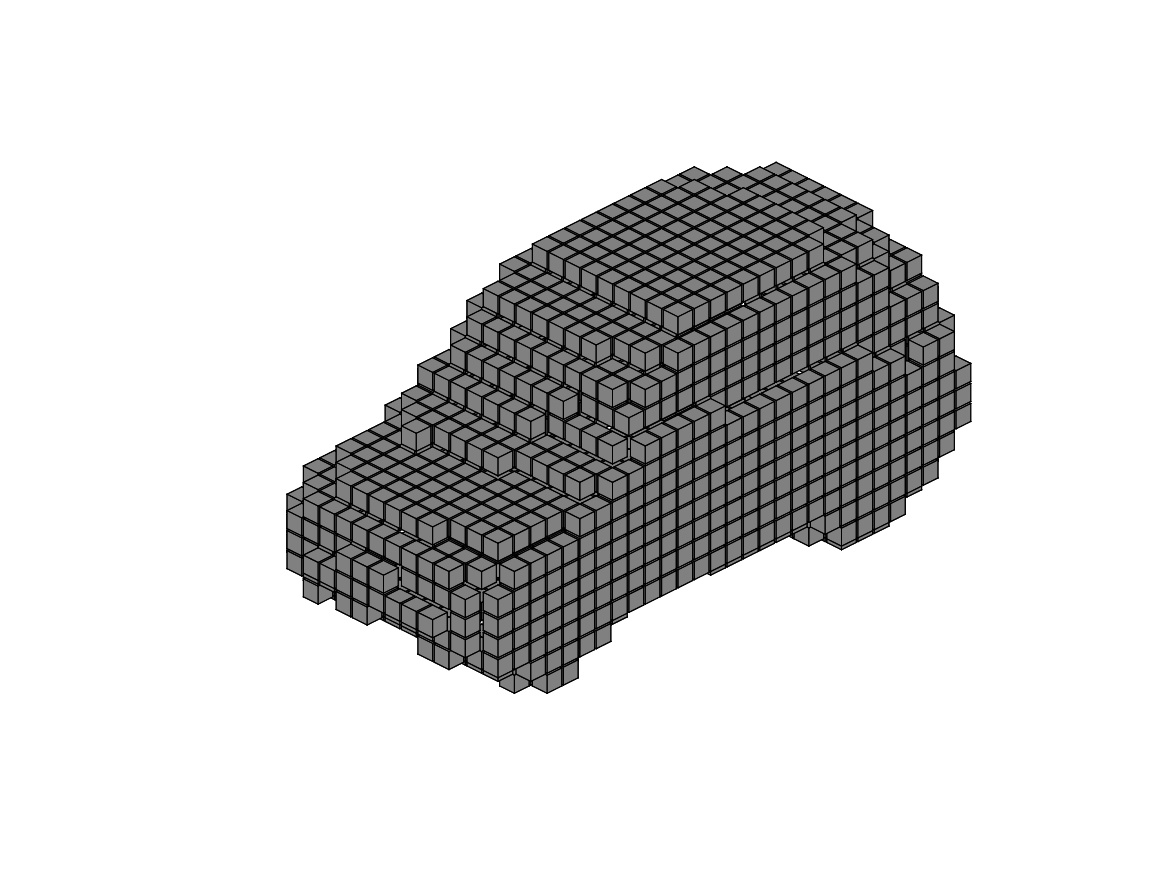
\includegraphics[width=3.75cm,trim={3.5cm 2.5cm 3.5cm 2.5cm},clip]{experiments/kitti/vae_occ_aml/15_long_statistics_combined/4_prediction_135}
    % };
    
    \node at (0, -12) {
      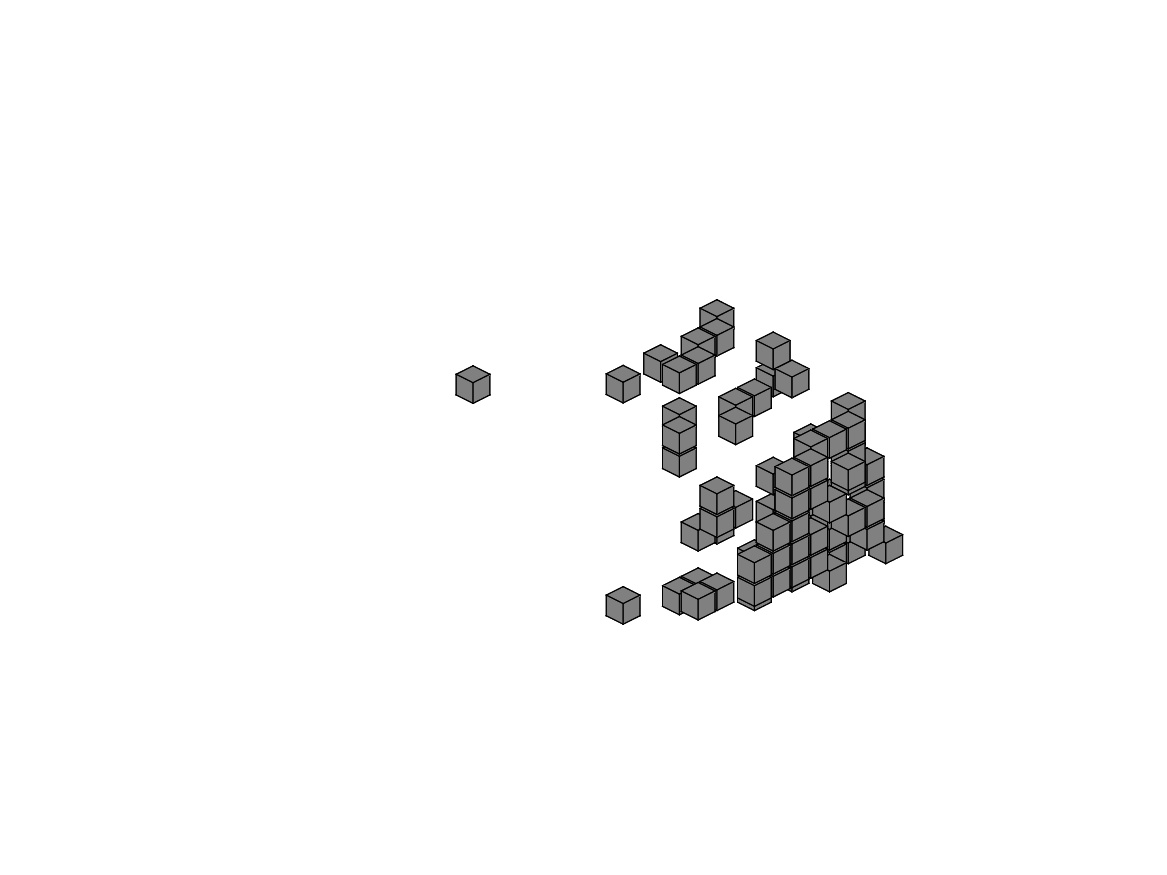
\includegraphics[width=3.75cm,trim={3.5cm 2.5cm 3.5cm 2.5cm},clip]{experiments/kitti/vae_occ_aml/15_long_statistics_combined/4_input_45}
    };
    \node at (3.5, -12) {
      \includegraphics[width=3.75cm,trim={3.5cm 2.5cm 3.5cm 2.5cm},clip]{experiments/kitti/vae_occ_aml/15_long_statistics_combined/4_prediction_45}
    };
    \node at (7, -12) {
      \includegraphics[width=3.75cm,trim={3.5cm 2.5cm 3.5cm 2.5cm},clip]{experiments/kitti/baseline/moderate_15/4_prediction_45}
    };

    \node at (0, 1.75) {Input};
    \node at (3.5, 1.75) {\AML};
    \node at (7, 1.75) {Baseline};
  \end{tikzpicture}

  % TODO short caption
  \caption{Comparison of \AML and the supervised baseline on KITTI; here,
  \AML uses occupancy only and we show the observed points and the predicted shapes
  in voxelized form. For both, we show 2 distinct viewpoints. For \AML we show
  two examples. For the latter, we also show the predicted shape using the supervised
  baseline to illustrate that \AML still misses details, \eg along the root.}
  \label{fig:experiments-kitti-aml-2}
\end{figure}
\begin{figure}
  \centering
  \begin{tikzpicture}
    \node at (0, 0) {
      \includegraphics[width=3.75cm,trim={3.5cm 2.5cm 3.5cm 2.5cm},clip]{experiments/kitti/vae_occ_sdf_aml/15_statistics_combined_075/0_input_45}
    };
    \node at (3.5, 0) {
      \includegraphics[width=3.75cm,trim={3.5cm 2.5cm 3.5cm 2.5cm},clip]{experiments/kitti/vae_occ_sdf_aml/15_statistics_combined_075/0_prediction_45}
    };
    \node at (8, 0) {
      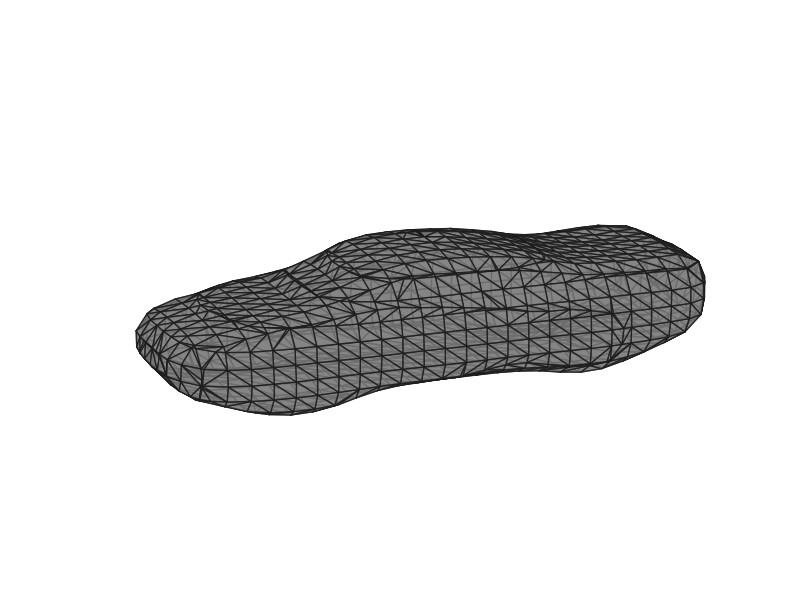
\includegraphics[width=3.75cm,trim={1cm 3cm 1cm 3cm},clip]{experiments/kitti/vae_occ_sdf_aml/15_statistics_combined_075/0_prediction}
    };
    
    \node at (0, -3) {
      \includegraphics[width=3.75cm,trim={3.5cm 2.5cm 3.5cm 2.5cm},clip]{experiments/kitti/vae_occ_sdf_aml/15_statistics_combined_075/1_input_45}
    };
    \node at (3.5, -3) {
      \includegraphics[width=3.75cm,trim={3.5cm 2.5cm 3.5cm 2.5cm},clip]{experiments/kitti/vae_occ_sdf_aml/15_statistics_combined_075/1_prediction_45}
    };
    \node at (8, -3) {
      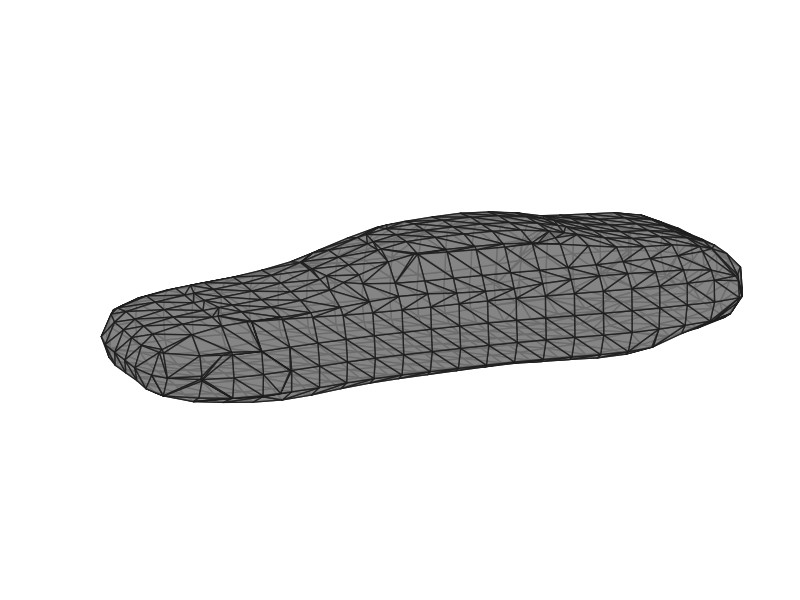
\includegraphics[width=3.75cm,trim={1cm 3cm 1cm 3cm},clip]{experiments/kitti/vae_occ_sdf_aml/15_statistics_combined_075/1_prediction}
    };

    \node at (0, -3) {
      \includegraphics[width=3.75cm,trim={3.5cm 2.5cm 3.5cm 2.5cm},clip]{experiments/kitti/vae_occ_sdf_aml/15_statistics_combined_075/2_input_45}
    };
    \node at (3.5, -3) {
      \includegraphics[width=3.75cm,trim={3.5cm 2.5cm 3.5cm 2.5cm},clip]{experiments/kitti/vae_occ_sdf_aml/15_statistics_combined_075/2_prediction_45}
    };
    \node at (8, -3) {
      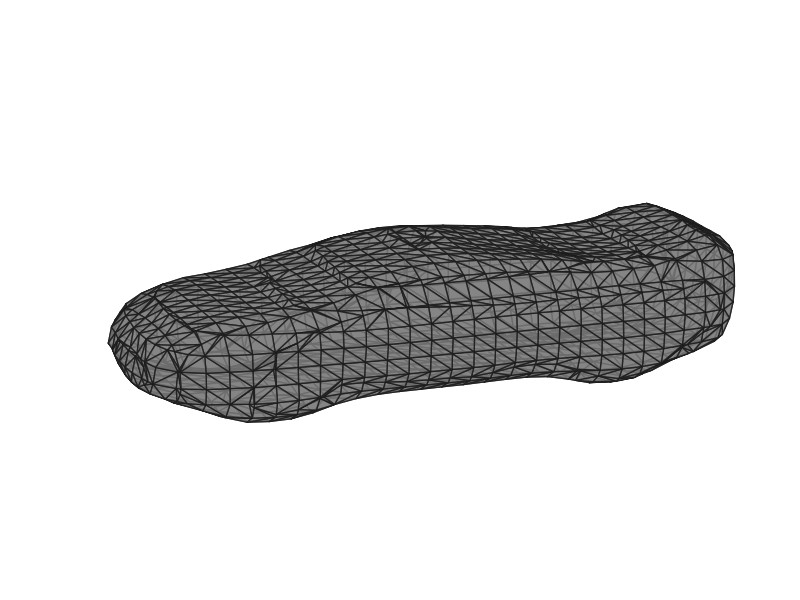
\includegraphics[width=3.75cm,trim={1cm 3cm 1cm 3cm},clip]{experiments/kitti/vae_occ_sdf_aml/15_statistics_combined_075/2_prediction}
    };
    
    \node at (0, 1.85) {input};
    \node at (3.5, 1.85) {prediction};
    \node at (8, 1.85) {mesh};
  \end{tikzpicture}

  % TODO short caption
  \caption{3D vsualizations of the predicted shapes using \AML predicting
  both occupancy and signed distance functions. The meshes on the right
  were derived using marching cubes.}
  \label{fig:experiments-kitti-aml-3}
\end{figure}


Using \AML, we are able to obtain reasonable shape completions from the
noisy observations. As shape prior, we re-trained the model used for ShapeNet
on all $40992$ samples from both training sets, \cf Table
\ref{table:experiments-shapenet-datasets}. In Figure
\ref{fig:experiments-kitti-aml-1} we first show
the observations, \ie observed points and free space, together with
the shape predictions for several examples from the validation set.
We also show the influence of using the weights from Equation
\eqref{eq:experiments-3d-weights} as well as training the prior on the combined
ShapeNet training sets.
As expected, using the weighted
loss has significant influence on the quality of the predicted shapes. In addition,
we also notice the benefit of having more training data for the prior. For the remaining
discussion we always use the weights as well as the stronger prior.
In Figure \ref{fig:experiments-kitti-aml-2} we show 3D visualizations
corresponding to the voxelized observations and the predicted shapes.
We find that the predicted shapes match the observed points rather well
and clearly depict cars. However, the predictions still miss a considerable
level of detail around the wheels and the roof. This can be seen as the
trade-off between noise robustness,
integrated through a strong prior, and detail-orientation.
Surprisingly, the predicted shapes look better than on the \hard ShapeNet-based
dataset, \ie Figure \ref{fig:experiments-shapenet-aml-qual-2}. This confirms our
intuition that the observations extracted from KITTI are slightly easier.
%In the conclusion, specifically Figure \ref{fig:conclusion}, we also show that
%the predicted shapes with the original scene reasonably well.
Overall, \AML is able to correctly predict orientation and rough shape
of the observed cars but also leaves room for improvement regarding details.

We also used a ShapeNet prior trained on both occupancy and signed distance
functions. However, we found the results to be slightly worse compared to
ShapeNet. As before, we suspect that longer training times and fine-tuning the
hyper parameters would be necessary to improve results. Nevertheless,
Figure \ref{fig:experiments-kitti-aml-3}
shows some examples of the predictions both in the form of occupancy grids
and meshes. As in the \hard case on ShapeNet, the prior
seems to favor small and thin cars. This tendency is emphasized by
the meshes derived using marching cubes and might be explained
by the uncertainty involved when reconstructing details such as wheels and roof.
Again, we can conclude that signed
distance functions, while being advantageous for deriving meshes, are more
difficult to learn in a weakly-supervised setting.

\subsection{Supervised Baseline}

We also investigated to which extent the supervised baseline from Section
\ref{sec:experiments-shapenet-supervised-baseline} is able to generalize to KITTI.
Figure \ref{fig:experiments-kitti-aml-2} shows qualitative results when
applying the learned model to KITTI observations. As can be seen, the model
predicts reasonable cars. In contrast to \AML,
the supervised model has no troubles predicting details along or the roof
or wheels. For some samples, however,
the predictions look very similar. Overall, the supervised baseline
appears to predict slightly more coherent shapes; but an exact evaluation and
comparison is not possible without ground truth annotations.
Overall, we find that there does not seem to be a significant gap between
\AML and the supervised baseline in terms of the visual quality of
the corresponding predictions.

\subsection{Discussion}

In the end, we can conclude that \AML is able to perform shape completion even under
real conditions as illustrated on KITTI. We also found that the supervised baseline
generalizes surprisingly well. However, compared to the supervised baseline,
\AML requires significantly less supervision. We find that using occupancy grids only,
we are able to recover slightly more detail compared to signed distance functions
as shape representation. The latter, however, allows to derive comparably smooth
meshes. As discussed before, we were not able to explore the full design space
regarding architectures, hyper-parameters and training. We expect \AML
using signed distance functions to show improved performance with increased
training time and optimized hyper parameters; however, we can only leave these
experiments for future work. Additionally, we could only judge results
qualitatively. While quantitative results are provided for ShapeNet, we do not
believe that these can be transferred one-to-one to KITTI. In particular,
we think the observation model used for ShapeNet does not completely match the true
observation model underlying KITTI. In conclusion, we are satisfied by the
demonstrated shape completion performance on KITTI and are looking forward to
future experiments in order to improve the proposed approach.

